\documentclass[11pt]{article}

\usepackage[a4paper]{geometry}
\geometry{left=2.0cm,right=2.0cm,top=2.5cm,bottom=2.5cm}

\usepackage{comment}
\usepackage{booktabs}
\usepackage{graphicx}
\usepackage{diagbox}
\usepackage{amsmath,amsfonts,graphicx,amssymb,bm,amsthm}
%\usepackage{algorithm,algorithmicx}
\usepackage[ruled]{algorithm2e}
\usepackage[noend]{algpseudocode}
\usepackage{fancyhdr}
\usepackage{tikz}
\usepackage{graphicx}
\usetikzlibrary{arrows,automata}
\usepackage{hyperref}
\usepackage{physics}
\usepackage{ctex}

\makeatletter
\newcommand{\rmnum}[1]{\romannumeral #1}
\makeatother

\setlength{\headheight}{14pt}
\setlength{\parindent}{0 in}

\newtheorem{theorem}{Theorem}
\newtheorem{lemma}[theorem]{Lemma}
\newtheorem{proposition}[theorem]{Proposition}
\newtheorem{claim}[theorem]{Claim}
\newtheorem{corollary}[theorem]{Corollary}
\newtheorem{definition}[theorem]{Definition}

\newenvironment{question}[2][Question]{\begin{trivlist}
\item[\hskip \labelsep {\bfseries #1}\hskip \labelsep {\bfseries #2.}]}{\hfill$\blacktriangleleft$\end{trivlist}}
\newenvironment{answer}[1][Answer]{\begin{trivlist}
\item[\hskip \labelsep {\bfseries #1.}\hskip \labelsep]}{\hfill$\lhd$\end{trivlist}}

\newcommand\E{\mathbb{E}}

\def\onedot{$\mathsurround0pt\ldotp$}
\def\cddot{% two dots stacked vertically
  \mathbin{\vcenter{\baselineskip.67ex
    \hbox{\onedot}\hbox{\onedot}}%
  }}%
\def\cdddot#1{% three dots 
  \mathbin{\vcenter{\baselineskip.67ex
    \hbox{\onedot}\hbox{\onedot}\hbox{\onedot}%
  }}%
}


\title{Homework Set \#1}
\usetikzlibrary{positioning}

\begin{document}

    \pagestyle{fancy}
    \lhead{}
    \chead{}
    \rhead{GAMES 001, 2024 Spring}

    \begin{center}
        {\LARGE \bf Homework \#2}\\
        {Due: 2024-4-30 00:00 \quad$|$\quad 4 Questions, 100 Pts}\\
        {Name: JS}
    \end{center}
    \begin{question}{1 (20') (欧拉角表示)}~
    试证明内旋效果等价于颠倒顺序后的外旋效果 (课件第29页)。具体地,试证明按照 $x-y^{\prime}-z^{\prime\prime}$ 依次转动 $\alpha,\beta,\gamma$ 的内旋效果与按照 $z-y-x$ 依次转动 $\gamma,\beta,\alpha$ 的外旋效果等价。
    \\
    \\
    证明:在内旋时$R_{y^\prime}$等价于先将绕$R_x$旋转后的新坐标系旋转$R_{x}^{-1}$为基坐标系,然后再进行旋转,最后恢复为新坐标系即
    \[R_{y^\prime} = R_{x}^{-1} R_y R_{x}\]
    同理可得$R_{z^{\prime\prime}} = ({ R_x R_{y^\prime}})^{-1} R_z R_x R_{y^\prime}$,综上,我们有:
    \[R_x R_{y^\prime} R_{z^{\prime\prime}} = R_x  R_{x}^{-1} R_y R_{x} ({ R_x R_{y^\prime}})^{-1} R_z R_x R_{y^\prime}\]
    \[ = R_z R_y R_x\]
    因此得证。
  
  \end{question}
    
  \begin{question}{2 (20') (轴角表示、四元数表示)}~
    试证明轴角表示下的相对旋转插值(课件第 37 页)与四元数表示的 Slerp 插值(课件第 52 页)等价。具体来说,你需要推导出两种插值方法在$t$时刻的旋转轴$\bm{u}_t$和旋转角度$\theta_t$是相同的,从而得到二者的旋转矩阵$\mathbf{R}_t$相同。
    \\
    \\
    证明:
  在轴角表示中,一个旋转可以表示为绕一个单位旋转轴\( \mathbf{u} \)旋转\( \theta \)度。给定两个旋转\( \mathbf{R}_0 \)和\( \mathbf{R}_1 \),它们的差异可以通过旋转\( \Delta\mathbf{R} = \mathbf{R}_1\mathbf{R}_0^{T} \)来表示,然后将\( \Delta\mathbf{R} \)转换为轴角表示\( (\mathbf{u}, \Delta\theta) \)。通过固定旋转轴\( \mathbf{u} \),可以通过对旋转角度\( \Delta\theta \)进行线性插值来实现旋转的插值,即:
  \[ \theta_t = t(\Delta\theta) \]

  四元数是一种表示空间旋转的方法,它避免了万向锁问题并且可以很方便地用于插值。对于两个旋转四元数\( q_1 \)和\( q_0 \),它们之间的Slerp插值定义为:
    
  \[ q_t = \frac{\sin((1-t)\theta)}{\sin\theta}q_0 + \frac{\sin(t\theta)}{\sin\theta}q_1 \]
  \[
   q_t = (\frac{1}{2} \cos {t \theta} , \frac{1}{2} \sin{ t \theta} \vb{u})
  \]
    
  其中,\( \theta \)是\( q_1 \)和\( q_2 \)之间的夹角,可以通过它们的点积计算得到。 
  
  可知轴角和四元数的插值过程中的旋转角度都是$t \theta$, 并且轴角表示中的旋转轴\( \mathbf{u} \)直接转换为四元数表示时,成为四元数旋转部分的方向,而Slerp插值保持两个四元数旋转部分方向的一致性。因此,插值过程中旋转轴不变。

  综上得证.

  
  \end{question}
    
    \begin{question}{3 (20') (四元数表示)}~
    试证明四元数的Slerp公式(课件第52页)。具体地,已知如下图所示,四元数 $v_0$ 与 $v_1$ 的夹角为 $\theta$,我们希望用 $v_0$ 和 $v_1$ 线性插值出四元数 $v_t$,即:
    $$
    v_t = \alpha v_0 + \beta v_1
    $$
    使得 $v_0$ 与 $v_t$ 的夹角为 $t\theta$,请证明 $\alpha = \frac{\sin ((1-t)\theta)}{\sin(\theta)}, \beta = \frac{\sin(t\theta)}{\sin(\theta)}$。
    \begin{figure}[h]
        \centering
        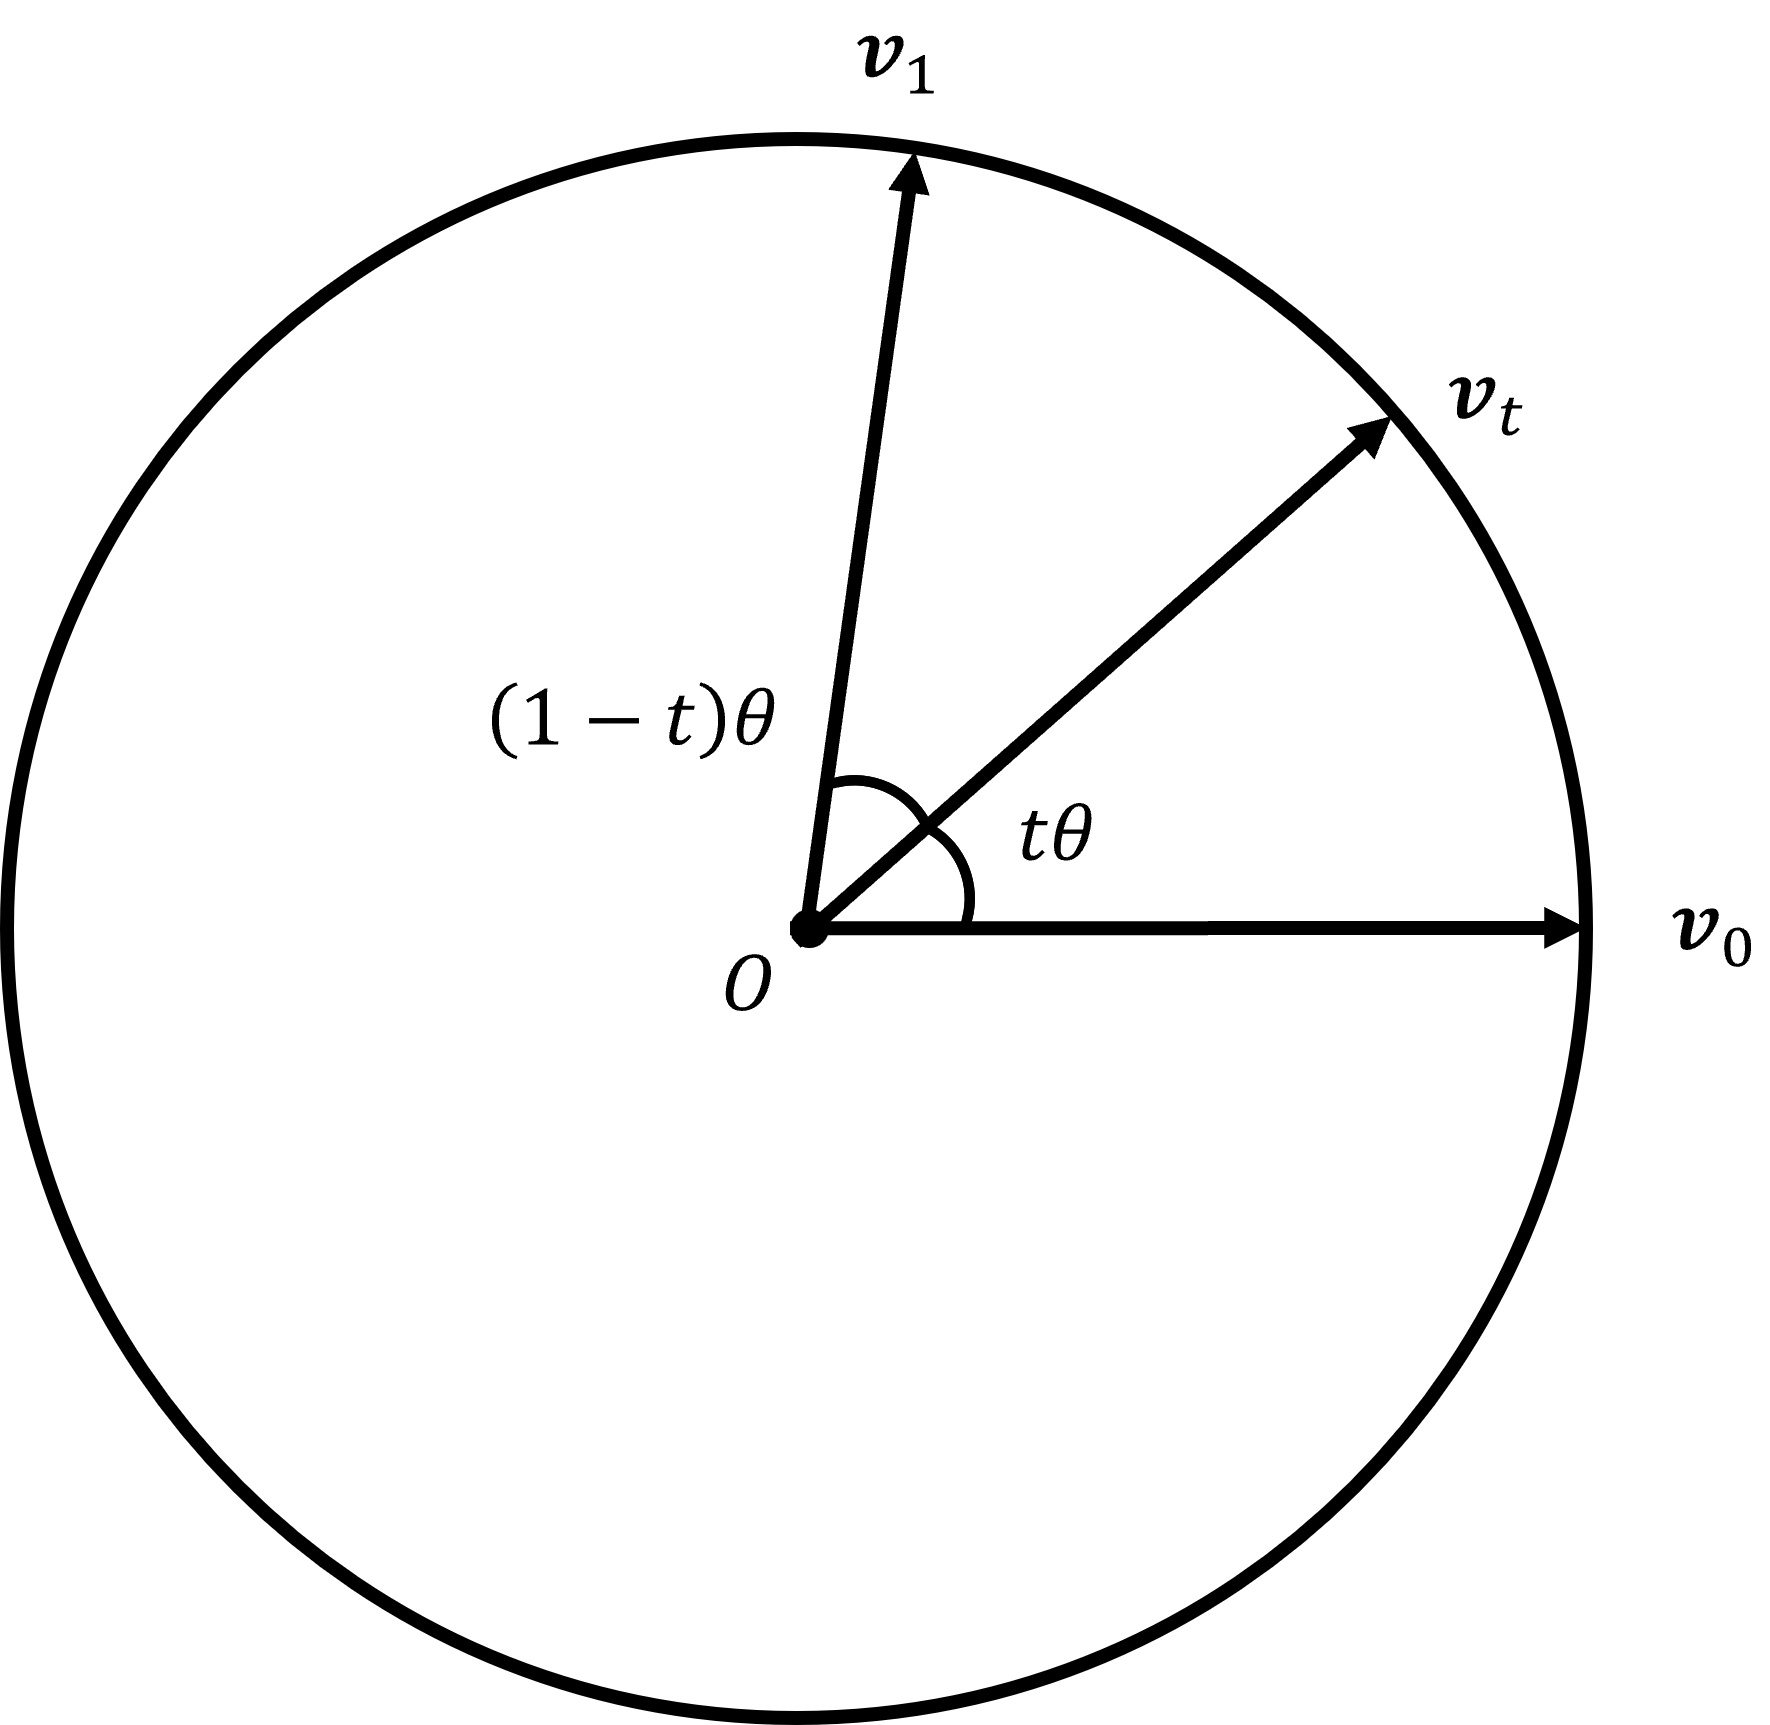
\includegraphics[width=0.25\textwidth]{slerp.png}
        \label{fig:my_label}
    \end{figure}
    \\
    \\
    证明:
    对$v_t = \alpha v_0 + \beta v_1$两边同时乘以$v_0$得到$v_0 \cdot v_1 = \alpha v_0 \cdot v_0 + \beta v_0 \cdot v_1$,对该式两边同取$\cos$
    可得
    \[\cos{(t \theta)}  = \alpha +\beta \cos{\theta}\]
    对$v_t = \alpha v_0 + \beta v_1$两边同时乘以$v_1$同理可得
    \[\cos{((1 - t) \theta)}  = \alpha \cos{\theta} +\beta \]
    为了求解\(\alpha\) 和 \(\beta\), 
    从第一个式子
    \[\alpha = \cos{(t \theta)} - \beta \cos{\theta}\]
    将 \(\alpha\) 带入第二个式子:
    \[\cos{((1 - t) \theta)} = (\cos{(t \theta)} - \beta \cos{\theta}) \cos{\theta} + \beta\]
    化简求 \(\beta\), 得到:
    \[\beta = \frac{\sin(t\theta)}{\sin(\theta)}\]
    将 \(\beta\) 带回求 \(\alpha\), 得到:
    \[\alpha = \frac{\sin((1-t)\theta)}{\sin(\theta)}\]
    \end{question}
\end{document}